\documentclass{report}
%\usepackage{fullpage}
\usepackage{parskip}
\usepackage{titlesec}
\usepackage{xcolor}

\usepackage{algorithm}
\usepackage[noend]{algpseudocode}
\algnewcommand{\LineComment}[1]{\State \(\triangleright\) #1}
\makeatletter
\def\BState{\State\hskip-\ALG@thistlm}
\makeatother
\usepackage{comment}
\usepackage{inputenc}
\usepackage{csquotes}
\usepackage{float}
%\excludecomment{figure}
\usepackage[backend=biber,maxcitenames=1]{biblatex}
\bibliography{library}
\renewbibmacro{in:}{}
\usepackage[]{graphicx}
\graphicspath{{img/}}
\usepackage{lmodern}
\renewcommand{\baselinestretch}{1.02}
\usepackage{xargs}                      % Use more than one optional parameter in a new commands
\usepackage[]{xcolor}  % Coloured text etc.
\usepackage[colorinlistoftodos,prependcaption,textsize=tiny]{todonotes}
%\newcommand\todo[1]{\textcolor{red}{#1}}
\newcommandx{\unsure}[2][1=]{\todo[linecolor=red,backgroundcolor=red!25,bordercolor=red,#1]{#2}}
\usepackage{graphicx}
\usepackage[space]{grffile}
\usepackage{latexsym}
\usepackage{textcomp}
\usepackage{longtable}
\usepackage{multirow,booktabs}
\usepackage{amsfonts,amsmath,amssymb}
% You can conditionalize code for latexml or normal latex using this.
\newif\iflatexml\latexmlfalse
\usepackage[english]{babel}
\DeclareMathOperator*{\argmin}{arg\,min}
\DeclareMathOperator*{\argmax}{arg\,max}
\usepackage{sectsty}
\allsectionsfont{\normalfont\scshape}
\usepackage{fancyhdr}
\pagestyle{fancyplain}
\fancyhead{}											% No page header
\fancyfoot[L]{}											% Empty 
\fancyfoot[C]{}											% Empty
\fancyfoot[R]{\thepage}									% Pagenumbering
\renewcommand{\headrulewidth}{0pt}			% Remove header underlines
\renewcommand{\footrulewidth}{0pt}				% Remove footer underlines
\setlength{\headheight}{13.6pt}
\PassOptionsToPackage{hyphens}{url}
%\usepackage{hyperref}
\usepackage{url}
%\usepackage{hyperref}
%\def\UrlBreaks{\do\/\do-}

\title{Thesis: Machine Learning-based Indoor Localization for Micro
  Aerial Vehicles}
\author{Volker Strobel}
\date{\today}

\begin{document}
\maketitle
\begin{abstract}
  Widespread applications, ranging from surveillance to search and
  rescue operations, make Micro Air Vehicles (MAVs) versatile
  platforms. However, MAVs have limited processing power due to their
  small size and cannot fall back on standard localization techniques
  in the indoor environment. Therefore, the ubiquitous use of MAVs is
  still impeded. To address this issue, an efficient onboard
  localization technique using machine learning was developed in the
  scope of this thesis.
  % The development, software and hardware implementation, and
  % results of the localization system are presented.

  The vision-based approach estimates $x,y$-coordinates within a known
  and modifiable indoor environment. Its computational power is
  scalable to different platforms, trading off speed and
  accuracy. Histograms of textons---small characteristic image
  patches---are used as features in a $k$-Nearest Neighbors ($k$-NN)
  algorithm. Several possible $x,y$-coordinates that are outputted by
  this regression technique are forwarded to a particle filter to
  neatly aggregate the estimates and solve positional ambiguities.
  % Promising results were obtained for all tasks: waypoint
  % navigation, accurate landing, and stable hovering in the indoor
  % environment.
  To predict the performance of the proposed algorithm in different
  environments an evaluation technique is developed. It compares
  actual texton histogram similarities to ideal histogram similarities
  based on the distance between the underlying $x,y$-positions. The
  technique assigns a loss value to a given set of images, allowing
  for comparisons between different environments and positions within
  the environment. To compare maps before modifying an environment, a
  software tool was created that simulates synthetic images that could
  be taken during an actual flight.

%The
%best one, the worst one and the one with median loss were printed out
%to compare their performance in the real-world. In fact, the results
%could be replicated on these maps.

  We conducted several flight tests to evaluate the performance of the
  approach. A comparison of the localization technique with the ground
  truth showed an average error of 50\,cm. In a triggered landing
  setting, the MAV correctly landed in specified areas, in ten out of
  ten trials. The method was tested on 46 high-resolution images to
  identify well-performing maps.

%The development, software and hardware
%implementation, and results of the localization system are presented.
%The estimates of the proposed system are compared to the ground truth in five on-ground and two
%in-flight experiments with promising results.

  The presented approach is based on three pillars: (i) a shift of
  processing power to a pre-flight phase to pre-compute
  computationally complex steps, (ii) lightweight and adaptable
  algorithms to ensure real-time performance and portability to
  different platforms, (iii) modifiable environments that can be
  tailored to the proposed algorithm. These pillars can build a
  foundation for efficient localization in various GPS-denied
  environments.
\end{abstract}
\chapter{Introduction}
\label{chap:introduction}

In the world of automation, micro aerial vehicles (MAVs) provide
unprecedented perspectives for domestic and industrial
applications. They can serve as mobile surveillance cameras, flexible
transport platforms, or even as waiters in restaurants. However,
indoor employment of these vehicles is still hindered by the lack of
real-time position estimates. The focus of this thesis is, thus, the
development of accurate and fast indoor localization for MAVs
combining computer vision and machine learning techniques.

%Many crimes over the last decades have been solved thanks to footage
%captured by surveillance cameras. However, stationary cameras can be
%easily manipulated or avoided once it is known where they are
%located. One possible solution may be the use of micro aerial vehicles
%(MAVs) for surveillance. To date, indoor employment of these vehicles
%is still hindered by several limitations. The focus of this thesis is,
%thus, the development of accurate and fast indoor localization for
%MAVs combining computer vision and machine learning techniques.

Since precision and reliability are crucial for safe flight,
autonomous indoor navigation of an MAV is a challenging task. While
unmanned aerial vehicles (UAVs) for outdoor usage can rely on the
global positioning system (GPS), this system is usually not available
in confined spaces and would not provide sufficiently accurate
estimates in cluttered environments.  If sufficient computational and
physical power is available, a typical approach to estimate a UAV's
position is by using active laser
rangefinders~\cite{grzonka2009towards,bachrach2009autonomous}.
Although this approach is used in some simultaneous localization and
mapping (SLAM) frameworks, it is usually not feasible for MAVs because
they can carry only small payloads. A viable alternative are passive
computer vision techniques. Relying on visual information scales down
the physical payload since cameras are often significantly lighter
than laser
rangefinders~\cite{blosch2010vision,angeli20062d,ahrens2009vision}.
Additionally, many commercially available drones are already equipped
with cameras.

Figure~\ref{fig:highleveloverview} summarizes the proposed
algorithm. In contrast to other existing approaches, it does not rely
on additional information, such as data from the inertial measurement
unit (IMU). The only required tool is a camera, which minimizes
possible points of failure. Cameras are lightweight and robust to many
external influences, such as magnetic fields.

\begin{figure}[h!]
\begin{center}
\includegraphics[width=0.7\columnwidth]{nutshell}
\caption{{\label{fig:highleveloverview} The figure illustrates the
    proposed system from a high-level perspective. An image
    feature---the texton histogram---is extracted from the current
    camera image of the UAV. The feature vector is forwarded to a
    machine learning model that uses a $k$-Nearest Neighbors algorithm
    to output $x,y$-position estimates. These estimates are passed to
    a particle filter, which filters position estimates over time and
    outputs a final position estimate (green circle). The expected
    loss shows regions in the map where a lower accuracy is
    expected. The average expected loss can be used as ``fitness
    value'' of a given map.%
  }}
\end{center}
\end{figure}

However, this reduced physical payload is not without cost: it must be
traded off against the higher computational payload for the onboard
CPU. Vision-based position estimation is usually a time-consuming and
memory-intense procedure.  For example, a standard technique for 3D
pose estimation extracts keypoints of the current camera image and a
map image and then determines a homography between both keypoint
sets. While this approach has been used for visual SLAM for
MAVs~\cite{blosch2010vision}, the pipeline for accurate feature
detection, description, matching, and pose estimation is
CPU-intensive~\cite{kendall2015posenet}.  One way to overcome
this problem is to process the data on a powerful external processor
by establishing a wireless connection between the MAV and a ground
station. Such off-board localization techniques often lack the
versatility to function in changing environments, though, due to
factors---such as the bandwidth, delay, or noise of the wireless
connection---interfering with the system's reliability.

In the approach proposed in this thesis, computational power will be
shifted to an offline training phase to achieve high-speed during live
operation. In contrast to visual SLAM frameworks, this project
considers scenarios in which the environment is known beforehand or
can be even actively modified. The environment is non-dynamic and
planar, therefore, the UAV will make use of texture on the bottom or
ceiling of the environment. This opens the door for improving the
proposed algorithm by changing the map. On the basis of desired
characteristics of a given map, an evaluation technique was developed
that determines the suitability of an environment for the proposed
approach. This technique allows for spotting distant regions with
similar image features, which could lead to deteriorated
performance. The evaluation can be performed using a given map image
or recorded images during flight. In the former case, synthetic images
will be generated from the map image that simulate images taken during
flight.

It uses a rather simple stimulus-response behavior to estimate the
position, which circumvents the requirement to store a map in the
UAV's `mind'. To assign $x,y$-coordinates to images in a training set,
keypoints in the current image and a map image are detected. This is
then followed by finding a homography---a perspective
transformation---between them to locate the current image in the
map. In the next step, the complexity of these images is reduced by
\emph{sparse encoding}: images are represented by determining their
histogram of textons---small characteristic image
patches~\cite{varma2005statistical}.  New images can then also be
encoded by texton histograms and matched to images with known
$x,y$-positions using the $k$-Nearest Neighbors ($k$-NN)
algorithm. The computational effort of the approach can be adjusted by
modifying the amount of extracted patches, resulting in a trade-off
between accuracy and execution frequency. While the $k$-NN algorithm
is one of the simplest machine learning algorithms, it offers several
advantages: it is non-parametric, allowing for the modeling of
arbitrary distributions. Its capability to output multiple predictions
with an associated confidence allows for neat integration with the
proposed particle filter. Finally, computational complexity can be
modified by changing the size of the datasets.

The goal is to estimate $x,y$-coordinates in real-time and on-board of
the UAV. It is assumed that the UAV flies at an approximately constant
height, such that the estimation of height is not necessary.  It is
intended to further reduce the size of MAVs to that of an insect,
hence necessitating lightweight and scalable position estimation
algorithms.

\section{Contributions}
\label{sec:contributions}

The first contribution of this thesis is a machine learning-based
indoor localization system that runs in real-time on board of an MAV,
paving the way to a fully autonomous system. In contrast to existing
\emph{active} approaches, the proposed \emph{passive} approach only
uses a monocular downward-looking camera. Since computer vision-based
localization approaches yield noisy estimates, a variant of a particle
filter was developed that aggregates estimates over time to produce
more accurate predictions. It handles the estimates of the $k$-NN
algorithm in an integrative way and resolves position ambiguities. The
method is an absolute position system and does not suffer from error
accumulation over time.

The second contribution is a map evaluation technique that predicts
the suitability of a given environment for the proposed algorithm. To
this end, a synthetic data generation tool was developed that creates
random variations of an image. The tool simulates different viewing
angles, motion blur, and lighting settings; the generated synthetic
images are labeled with $x,y$-coordinates based on the 3D position of
the simulated camera model.

The developed software is made publicly available. It encompasses (i)
the localization algorithm as part of the Paparazzi project, which
consists of the texton-based approach in combination with a particle
filter (ii) software for augmenting an image with synthetic views,
(iii) a script for evaluating a map based on histograms and
corresponding $x,y$-positions.


\section{Research Questions}
\label{sec:researchquestions}

The research questions addressed in this thesis are:

\begin{itemize}
\item ``\emph{Can 2D positions be estimated in real-time using a
    machine learning approach on a limited processor in a modifiable
    indoor
    environment?}''  \vspace*{0.15cm}\\
  Real-time position estimates can pave the way for autonomous flight
  of MAVs in various indoor environments; pursuing an ``onboard
  design'' to make the MAV independent of an external ground station
  is an important step for security and versatility.
%\item Is accurate real-world localization regression possible when the
%  training data comprises synthetic data only?
\item \emph{``Can we predict the suitability of a given map for the proposed
  localization approach?''}  \vspace*{0.15cm}\\
  If a map can be evaluated before actually flying in this
  environment, the performance of the approach can be predicted and
  possible dangers prevented.
\end{itemize}

\section{Outline}
\label{sec:outline}

The remainder of this thesis is structured as follows.
Chapter~\ref{chap:relatedwork} surveys existing indoor localization
approaches related to this thesis. In Chapter~\ref{chap:methods}, the
developed texton-based approach is presented and its components, the
$k$-NN algorithm and the particle filter, are introduced. Details about
the synthetic data generation tool and map evaluation technique are
also given. Chapter~\ref{chap:analysis} describes the setup and
results of the on-ground and in-flight experiments. The results are
then discussed in Chapter~\ref{chap:discussion}. Finally, we draw our
conclusions and indicate future research directions in
Chapter~\ref{chap:conclusion}.

\chapter{Related Work}
\label{chap:relatedwork}

This chapter will discuss advantages and disadvantages of different
approaches for indoor localization and contrast them to the proposed
method. While a wide range of methods for indoor localization exists,
from laser range scanners over depth cameras to RFID tag based
localization, only methods that use the same technical and conceptual
setup---coordinate estimation with a monocular camera---are
discussed. Two types of localization are distinguished: local
techniques and global techniques~\cite{fox1999monte}. Local techniques
need an initial reference point and estimate a robot's coordinates
based on the change in position over time. Once they lost track, the
robot's position can typically not be recovered. The approaches also
suffer from ``drift'' since errors are accumulating over time. Global
techniques are more powerful and do not need an initial reference
point. They can recover when temporarily losing track and address the
\emph{kidnapped robot problem}, in which a robot is carried to an
arbitrary location~\cite{engelson1992error}.

Comparing the accuracy and run-time of different localization methods
is difficult: target systems and test environments are often too
different to draw comparisons. The annual Microsoft Indoor
Localization Competition aims at setting a standardized testbed for
comparing near real-time indoor location
technologies~\cite{microsoft}. However, since the competition does not
require lightweight platforms and allows the use of external
infrastructure such as WiFi routers, no vision-only approach has yet
been presented at the competition.

\section{Vision-based Localization Methods}

\subsection{Fiducial Markers}
\label{sec:fiducialmarkers}

Fiducial markers (Figure~\ref{fig:aruco}), which are often employed in
augmented reality
applications~\cite{kato1999marker,garrido2014automatic}, have been
used for UAV localization and
landing~\cite{eberli2011vision,bebop2015}. The markers encode
information by the spatial arrangement of black and white or colored
image patches. Their corners can be used for estimating the camera
pose at a high frequency. The positions of the markers in an image are
usually determined with \emph{local thresholding}. Local thresholding
is a simple method for separating objects---salient image
regions---from a background. Its output is a binary image with two
states: foreground (markers) and background. Marker positions are then
often further refined by removing improbable shapes, yielding an
adjusted version of possible marker
positions~\cite{aruco2014}. Various popular marker libraries exist,
including ArUco~\cite{aruco2014} and ARToolKit~\cite{kato1999marker}.

An advantage of fiducial markers is their widespread use, demonstrated
by several technically mature and open-source libraries. Given
adequate lighting conditions, markers can be used in a wide variety of
environments~\cite{hornecker2005using}. This makes them suitable for
indoor localization.  A drawback of the approach is that motion blur,
which frequently occurs during flight, can hinder the detection of
markers~\cite{albasiouny2015mean}. Furthermore, partial occlusion of
the markers through objects or shadows break the detection; each
marker needs to be fully in the camera
view~\cite{hornecker2005using}. Another downside is that markers might
be considered as visually unpleasant and may not fit into a product or
environmental design~\cite{chu2013halftone}. They offer little
flexibility, since one has to rely on predefined marker dictionaries;
additionally, marker-based approaches require to \emph{always} modify
the environment. Like most vision-based approaches, the detection of
markers is prone to changes in lighting conditions and may not work in
low-contrast settings~\cite{hornecker2005using}.

%There is no direct way to modify the time complexity of the algorithm.

% TODO: which errors have been achieved

\begin{figure}[h!]
\begin{center}
\includegraphics[width=0.252\columnwidth]{markers}
\caption{{\label{fig:aruco}
Examples of fiducial markers of the ArUco library.%
}}
\end{center}
\end{figure}

\subsection{Homography Determination \& Keypoint Matching}
\label{sec:keypointmatching}

A standard approach for estimating camera pose is detecting and
describing keypoints of the current view and a reference
image~\cite{se2002global}, using algorithms such as Scale-invariant
feature transform (\textsc{Sift})~\cite{lowe1999object}, followed by
finding a homography---a perspective transformation---between both
keypoint sets. A keypoint is a salient image location described by a
feature vector. Depending on the algorithm, it is
invariant to different viewing angles and scaling.\\
The \textsc{Sift} algorithm transforms an image into a set of image
features. It works in four subsequent stages using gray-scale images
as input:
\begin{enumerate}
\item \emph{Maxima detection:} The image is convolved with the
  \emph{Difference of Gaussian} blob detector. By varying the variance
  of the Gaussian distribution, the maxima---potential
  keypoints---across different scales and spaces can be detected.
\item \emph{Refinement of keypoints:} The potential keypoints are
  refined by removing maxima with small contrast and non-discriminative
  edges.
\item \emph{Orientation detection:} The keypoints are labeled with
  their orientation, expressed as angle in radians.
\item \emph{Keypoint description:} The local image gradients are
  transformed into a 128-element feature vector by describing pixels
  around a radius of a keypoint.
\end{enumerate}

To locate the current view in the reference image, keypoints from one
set are matched with their nearest neighbor in the other set using the
Euclidean distance between their feature vectors. Based on the matched
keypoint descriptions, a homography is calculated between the
coordinates of both keypoint sets. This allow for locating the current
view in the reference image. The calculation of homography matrix
($H$) needs at four keypoint matches between both images. Usually many
more points are available, leading to an overdetermined equation. The
solution to $H$ is then computed by minimizing the errors of between
all the projected keypoints in a least-square sense.

While this \emph{homography-based} approach is employed in frameworks
for visual Simultaneous Localization and Mapping (SLAM), the pipeline
of feature detection, description, matching, and pose estimation is
computationally complex~\cite{kendall2015posenet}. Therefore, ground
stations for off-board processing or larger processors are usually
needed for flight control.

% TODO:
% Where has the approach been used and is suitable for the proposed algorithm. 

\begin{figure}[h!]
\begin{center}
\includegraphics[width=0.448\columnwidth]{sift}
\caption{{Perspective transformation between keypoints of the current image (left) and the reference or map image (right).%
}}
\end{center}
\end{figure}

The approach has been employed for absolute localization for UAVs:
\citeauthor{blosch2010vision}~\cite{blosch2010vision} evaluate it on a
$3.5\,m \times 2\,m$ area and achieve a root mean square (RMS)
positional error below $10\,cm$ in $x,y,z$-direction. Calculations are
executed on a powerful ground station, which is connected to the UAV
with a USB cable. Subsequent research has brought the algorithm on
board of the UAV~\cite{achtelik2011onboard}, achieving a frequency of
10\,Hz with a 1.6 GHz onboard processor with 1 GB RAM. However, the
required processing power is still too complex for small
MAVs~\cite{de2009design}.

\subsection{Convolutional Neural Networks}

Convolutional neural networks (CNNs) are artificial neural networks
specialized for image processing~\cite{lecun1998gradient} and have
outperformed classical approaches in many computer vision
challenges~\cite{dosovitskiy2014discriminative}. They consist of
multiple neuron layers, which represent increasing levels of
abstraction~\cite{lecun1998gradient}. Usually, the training of such
networks requires a considerable amount of time, in the range of hours
and days. However, the prediction often takes only few milliseconds,
shifting computational effort from the test phase to the training
phase. CNNs been used as more robust alternative to \textsc{Sift} if
images are perturbed~\cite{dosovitskiy2014discriminative}, however,
with larger computation time.

In recent work, \citeauthor{kendall2015posenet} present the first
framework for regressing camera positions based on
CNNs~\cite{kendall2015posenet}. The authors claim that the approach is
robust to different lighting settings, motion blur, and varying camera
intrinsics.  The approach achieves an accuracy of approximately 50\,cm
in indoor environments with a spatial extent between
$2 \times 0.5 \times 1\,m^3$ and $4 \times 3 \times 1.5\,m^3$. While
the approach works remarkably fast on a modern desktop computer, it is
still computationally too involved for a limited processor.

\subsection{Optical Flow}
\label{sec:opticalflow}

Optical flow algorithms are biologically inspired methods for
navigation---taking inspiration from insects and
birds~\cite{ruffier2003bio}. They estimate the motion based on the
shift of corresponding image keypoints in successive images. The most
popular optical flow methods are gradient based approaches and
keypoint-based methods.
% and more specific methods have been put forth\todo{for example}.
Optical flow methods belong to the class of local localization
techniques and can only estimate the position relative to an initial
reference point. The approaches suffer from accumulating errors over
time and typically do not provide a means for correcting these errors.

\unsure{And conclude
  what?}\citeauthor{chao2013survey}~\cite{chao2013survey} compare
different optical flow algorithms for the use with UAV navigation. The
approaches are computationally rather
complex~\cite{mcguire2016local}. To render on-board odometry feasible
for small MAVs, \citeauthor{mcguire2016local}~\cite{mcguire2016local}
introduce a lightweight optical flow variant. The algorithm uses
compressed representations of images in the form of edge histogram to
calculate the flow.

\section{Texton-based Machine Learning Methods}
\label{sec:textonbasedapproaches}

Textons are small characteristic image patches that can be used as
image
features. \citeauthor{varma2005statistical}~\cite{varma2005statistical}
originally introduced textons for classifying different textures,
showing that they outperform computationally more complex algorithms,
like Gabor filters~\cite{varma2005statistical}. For the
classification, the approach compares texton histograms between a
training set and the test sample and the class of the closest training
sample is assigned to the test sample. To extract histograms in the
\emph{full sampling} setting, a small window---a kernel---is convolved
over all image positions and the frequency of textons is calculated.
Instead of convolving a kernel over the entire image, the kernel can
be applied at randomly sampled image
position~\cite{de2012sub}. %leading to similar texton histograms
                           %compared to the histograms when full
                           %sampling is used.
Modifying the number of samples allows for adjusting the computational
effort, resulting in a trade-off between accuracy and execution
frequency. A disadvantage is that it discards all information about
the spatial arrangement of textons---it does not make use of the
\emph{Where} of the information, just of the \emph{What}, which can
result in different images with similar histograms.

\citeauthor{de2009design}~\cite{de2009design} use textons as image
features to distinguish between three height classes during
flight. Using a nearest neighbor classifier, their approach achieves a
height classification error of approximately 22\,\% on a hold-out test
set.  This enables a flapping-wing MAV to roughly hold its height
during an experiment. In another work,
\citeauthor{de2012appearance}~\cite{de2012appearance} introduce the
\emph{appearance variation cue}, which is based on textons, for
estimating the proximity to objects~\cite{de2012appearance}.
% Since closer objects should have less variation, these objects
% should appear less varied.
Using this method, their MAV is able to avoid obstacles in a
$5m \times 5m$ office space and achieves an AUC of up to .97 on rather
distorted images.
%Additionally, it performs better than or, at least, equal to
%optical flow estimations.

\chapter{Methods}
\label{chap:methods}

This section describes the ideas behind the developed approach, the
hardware and software implementations, and the design of the
experiments.
% An overview of the entire process is sketched out in
% Figure~\ref{fig:overview}.
The approach is based on three ``pillars'': (i) a shift of processing
power to a pre-flight phase to pre-compute computationally complex
steps, (ii) lightweight and adaptable algorithms to ensure real-time
performance and portability to different platforms, (iii) modifiable
environments to get the most out of the approach. The pseudo code in
Algorithm~\ref{alg:trexton_run} shows a high-level overview of the
parts of the framework. Details about the parts of the framework and
the ``pillars'' will be given in separate sections. All developed
software is made publicly available, the corresponding links are given
in the respective sections.
\begin{algorithm}
    \caption{Run texton framework}
    \label{alg:trexton_run}
    \begin{algorithmic}[1]
      \Procedure{Run\_TreXton}{} \State $t \gets t+1$ \State
      $I_t \gets$ \Call{Receive\_Img\_from\_Camera}{} \State
%      $\widetilde{I_t} \gets$ \Call{Standardize\_Image}{$I_t$} \State
      $\mathcal{H}_t \gets$ \Call{Get\_Histogram}{$I_t$}
      \State $\mathbf{z}_t \gets$
      \Call{$k$-NN}{$\mathcal{H}_t$} \State $f_t^x, f_t^y \gets$
      \Call{Calc\_Flow}{$I_t$} \State $\mathcal{X}_t \gets$
      \Call{Particle\_Filter}{$\mathcal{X}_{t-1}, z_t^x, z_t^y, f_t^x,
        f_t^y$} \State $x_t, y_t \gets$
      \Call{Map\_Estimate}{$\mathcal{X}_t$} \State
%      \Call{Send\_Pos}{$x_t, y_t$}
      \EndProcedure
    \end{algorithmic}
  \end{algorithm}  
\section{Hardware and Software of the Platform}
\label{sec:hardware}

In our first approach, the commercially available Parrot AR.Drone2.0
was equipped with an Odroid XU-4 single board computer, a Logitech 525
HD webcam, a WiFi module. Figure~\ref{fig:comparison} shows the
setup. The camera images were processed on the more powerful Odroid
processor and the resulting $x,y$-estimates were sent over a USB data
link to the MAV flight controller. The Odroid processor has a full
operating system (Ubuntu 15.04) and allows for running arbitrary Linux
software.  However, the additional weight through the modifications of
the system resulted in unstable flight performance. Therefore, we
modified the system to execute the localization algorithm directly on
board of the MAV and not on the additional Odroid processor. To this
end, the software had to be ported from the high-level language Python
to the low-level language C without being able to rely on many
existing software libraries.  Finally, this removed the need for
additional payload and made flight performance very stable. Also, it
circumvented the effort of buying and attaching an external processor,
which can be another point of failure. Another advantages is that the
framework can be easily ported to any UAV supported by the paparazzi
software. The major disadvantage is that the on-board processors of
many MAVs have a lower performance than the Odroid processor.

We decided to use the quadcopter \emph{Parrot Bebop Drone} as
prototype for all our tests. Quadcopters allow for navigating in
arbitrary directions without changing their yaw angle. Modern
quadcopters show stable flight behavior and are eqipped
high-resolution cameras. The \emph{Parrot Bebop Drone} is equipped
with a lithium-ion polymer battery that allows for approximately 11
minutes flying time. The UAV's dimensions are
$28 \times 32 \times 3.6$\,cm and it weighs 400\,g. The UAV is
equipped with two cameras: a front camera and a downward-looking
bottom camera. The developed approach makes use of the bottom camera
only. This camera has a resolution of $640 \times 480$ pixels with a
frequency of 30 frames per second. The UAV's processor is a Parrot P7
dual-core CPU Cortex A9 with a tact rate of 800\,Mhz. It is equipped
with 8~GB of flash memory and runs a Linux operating system. The full
specifications of the UAV can be found at its official
website~\cite{bebop}.

The original Bebop software development kit was replaced with
Paparazzi. Paparazzi is an ``open-source drone hardware and software
project encompassing autopilot systems and ground station
software''~\cite{paparazzi}. Its modular approach allows for combining
functions regarding stabilization, localization, and control of UAVs.
The presented approach is implemented as module in Paparazzi's
computer vision framework. Since low-level routines like accessing
camera information or attitude control for different platforms are
already implemented in Paparazzi, the module can be readily used
across different platforms. Modules are written in the C programming
language and are cross-compiled on the host PC to make them suitable
for the UAV's processor. Afterwards, they are uploaded to the
microprocessor of the UAV, allowing for autonomous execution of the
compiled software. A downlink connection---from the UAV to the
groundstation---allows for monitoring the state of the aircraft, for
example information about speed, altitude, position, or battery
status.

While the goal of the presented system is to rely solely on onboard
processing, monitoring the system during evaluation on a ground
station is important. Figure~\ref{fig:gcs} shows the default ground
control station of Paparazzi. For collecting data, real-time
visualization of the position estimates and enabling future users to
keep track of the system states, a graphical user interface (GUI) has
been developed in the scope of this thesis. The GUI is displayed in
Figure~\ref{fig:gui}.
\begin{figure}[t]
\begin{center}
\includegraphics[width=0.7\columnwidth]{Gcs}
\caption{{\label{fig:gcs} The ground control station of the Paparazzi
    software. It displays information about the status of the UAV and
    allows for controlling the vehicle.%
  }}
\end{center}
\end{figure}
The GUI displays the position estimate of the developed framework, the
ground truth position based on OptiTrack, the texton histogram, the
Euclidean distances between OptiTrack and the system, the uncertainty
of the system, and the correlation between the uncertainty and the
Euclidean distance between the Optitrack and treXton estimates. The
GUI can be accessed using the \emph{Tool} menu in paparazzi.
\begin{figure}[t]
\begin{center}
\includegraphics[width=0.7\columnwidth]{gui-cut}
\caption{{\label{fig:gui} Screenshot of the GUI. It displays the
    position estimate of the developed framework, the ground truth
    position based on OptiTrack, the texton histogram, the Euclidean
    distances between OptiTrack and the system, and the uncertainty of
    the system (based on the spread of particles).%%
  }}
\end{center}
\end{figure}

\section{Pillar I: Label images with $x,y$-coordinates}
\label{sec:mapping}

% To exploit the advantages, and straighten out the disadvantages, we
% used the approach in a preprocessing step to obtain labeled training
% data of a known environment.  This allows to shift computational
% effort from the flight phase to a pre-flight phase---paving the way
% for autonomous flights of MAVs with limited processing power.

A main idea of the presented method is to shift computational effort
to a pre-flight phase. Since the MAV will be used in a fixed
environment, the results of these pre-calculations can be employed
during the actual flight phase. In this first step, the goal is to
label images with the physical $x,y$-position of the UAV at the time
of taking the image. Therefore, a method for obtaining the physical
position of the UAV is needed and GPS information is not available in
the indoor environment. One possible way to create the training set is
to align the images with high-precision position estimates from a
motion tracking system.
% Even low quality images can be mapped to the corresponding
% $x,y$-position.
The $x,y$-position is broadcast to the UAV via the ground station,
which is connected to the motion tracking system.  The data set is
created by saving the image with the corresponding position from the
motion tracking system on the MAV's hard disk.

The approach yields high-quality training sets since motion tracking
systems can track rigid bodies at a high frequency within an error of
few millimeters. The major disadvantages of the approach are that
motion tracking systems are usually expensive and time-consuming to
move to different environments.

As an alternative, we sought a low-budget and more flexible
solution. Of the presented approaches in Section~\ref{chap:methods},
the homography-based approach (Section~\ref{sec:keypointmatching})
promises the highest accuracy but also requires the highest processing
time. Since fast processing time is not relevant during the pre-flight
phase, the approach is well-suited for the problem.
% high matching quality for non-blurry images, it suffers from lacking
% robustness to noise and the high processing time requirements.  It
% is based on two associated cornerstones that are performed in an
% offline phase: the creation of a two-dimensional map and finding
% homographies homography.
The required image dataset can be obtained by using images obtained
during manual flight or by recording images with a hand-held
camera. For creating a map, the images from the dataset have to be
stitched together to get a hyperspatial image of the scene. The
stitched image has a higher resolution than the single images and
contains a greater range of detail.  Certain software packages allow
for orthorectifying the images by estimating the most probable viewing
angle based on the set of all images. However, since a
downward-looking camera is attached to the UAV, most images will be
roughly aligned with the z-axis, given slow
flight~\cite{blosch2010vision}.  For the stitching process, the
freeware software Microsoft Image Composite Editor (ICE) was
used~\cite{ice}. This closed-source software but does not publish
details about the used techniques. As an open-source alternative, the
panorama photo stitching software \emph{hugin} is available. In our
tests, Microsoft ICE yielded better quality results.\unsure{could show
image of hugin vs ICE}

Keypoints of the current image and the map image are detected and
described using the \textsc{Sift} algorithm. The keypoint sets are
further refined using Lowe's ratio test~\cite{lowe1999object}. This is
followed by a matching process, that identifies corresponding
keypoints between both images. The matching uses a 'brute-force'
matching scheme and every keypoint is compared to every other
keypoint. These matches allow for finding a homography between both
images. For determining the $x, y$-position of the current image, the
center of it is projected on the reference image using the homography
matrix. The pixel position of the center in the reference image can be
used to determine the real world position by transforming the pixel
coordinates to real-world coordinates, based on the scale factors
$C_x$ and $C_y$, with $C_x = \frac{width(W)}{width(I)}$ and
$C_y = \frac{height(W)}{height(I)}$, where $W$ is the real-world
dimension and $I$ the digital pixel image. This yields a dataset of
images, labeled with $x, y$ coordinates and the number of matches.

The stitching process can be time-consuming and error-prone. It can be
impeded by distortions and perspective transformations of the recorded
images. To circumvent the need for stitching together multiple images,
an image with high-resolution camera from a top view point can be
taken in some environments that captures the entire area. Yet another
method starts with an existing image and modifies the environment
accordingly---for example by painting the floor or printing
posters--to correspond to the image.
%In all cases, we will describe
%the environment as \emph{map image}.
The homography-based process already introduces noise into the
dataset, depending on the quality of the keypoint matches.
% The $x,y$-positions are of different quality depending on the used
% technique: homography-based, poster-based, or motion tracking-based.
\begin{figure}[h!]
\begin{center}
\includegraphics[width=0.448\columnwidth]{bestmap}
\caption{{\label{fig:orthomap}
This figure shows
    the created orthomap of a rather texture-rich floor. It is
    stitched together using 100 single images and represents a
    real world area of approximately $8\times8$ meters. Image
    distortions, non-mapped areas, and slightly skewed seams at
    several points are visible.%%
}}
\end{center}
\end{figure}

Instead of saving the images on the hard disk, the texton histograms
can be directly aligned with the $x,y$-positions.

\section{Pillar II: Texton-based Approach}
\label{sec:textons}

In this section, the core of the developed algorithm is described: the
implementation of the texton framework, consisting of the texton
dictionary generation, the extraction of the histograms, the
$k$-Nearest Neighbors ($k$-NN) algorithm, and the particle filter. The
dictionary of textons constitutes the base for determining the texton
histograms. These histograms are used as features in the $k$-NN
algorithm. The algorithm outputs possible $x,y$-coordinates for a
given image, which are forwarded to the particle filter to yield a
final position estimation.

\subsection{Texton Dictionary Generation}
\label{sec:text-dict-gener}

For learning a suitable dictionary for an environment, image patches
were clustered. The resulting cluster centers---the prototypes of the
clustering result---are the textons~\cite{varma2003texture}. The
clustering was performed using a competitive learning scheme with a
``winner-take-all strategy'', a simple variant of a Kohonen
network~\cite{kohonen1990self} with an empty set as neighborhood
function. In the beginning, the dictionary is initialized with
$n = 20$ random image patches from the first image, which form the
first guess for cluster centers. Then, a new image patch $x$ is
extracted and compared to each texton $d_j$ in the tentative
dictionary using the Euclidean distance. The most similar texton $d_r$
is the ``winner.'' This texton is then adapted to be more similar to
the current patch, by calculating the difference in pixel values
between the current images patch and the texton and updating the
texton with a learning rate of $\alpha = 0.02$:
\begin{align}
  d_r := d_r + \alpha (x - d_r)
\end{align}
The first 100 images of each dataset were used to generate the
dictionary. From each image, 1000 randomly selected image patches of
size $w \times h = 6 \times 6$ were extracted, yielding $N = 100\,000$
image patches in total that were clustered. An example of a learned
dictionary can be found in Figure~\ref{fig:dictionary}.

Different maps and environmental settings require different texton
dictionaries. If one would use the same dictionary for each map, it
might happen that the histogram has only a few non-zero elements, and
thus, cannot represent the variance in the map. While we set the
number of textons to $n = 20$ for all maps, this parameter is also
map-dependent, and ideally, if time allows, could be adapted to the
given map.

\begin{figure}[h!]
\begin{center}
\includegraphics[width=0.7\columnwidth]{dict}
\caption{{\label{fig:dictionary} The figures shows a dictionary
    consisting of 20 grayscale textons. The textons are six pixels
    high and six pixels wide.%
  }}
\end{center}
\end{figure}

\subsection{Histogram Extraction}
\label{sec:histogramextract}

The shift is accomplished by using a light-weight machine learning
approach instead of a computationally more complex algorithm, like a
homography-based approach
(Section~\ref{sec:keypointmatching}). Supervised machine learning
methods need a training set to find a mapping from features to target
values. In the presented approach, a training sample consists of a
texton histogram (Section~\ref{sec:textonbasedapproaches}) as feature
vector. The process for obtaining a texton histogram from an image is
described in Section~\ref{sec:textons}.

\subsection{$k$-Nearest Neighbors ($k$-NN) algorithm}
\label{sec:knn}
% TODO: Write that one could also use a more efficient data structure than simply a list

The $k$-Nearest Neighbors ($k$-NN) algorithm is the ``machine
learning-core'' of the developed algorithm. Taking a texton histogram
as input, the algorithm measures the distance of this histogram to all
histograms in the training dataset and outputs the $k$ most similar
training histograms and the corresponding $x,y$-positions.

% The similarity measure is a function that takes two samples as input
% and outputs a real value. We used the cosine similarity as
% similarity function, since it is bounded between 0 and 1. While
% other similarity measurements exists, the basic similarity
% measures---such as Euclidean distance---do not have a large impact
% on the results (Figure xxx). The choice of $k$ was based on the
% heuristic that XXX (TODO: write something like the sqrt of N or
% whatever) and on cross-validation.

The naive approach in $k$-NN regression calculates the mean of the $k$
outputs; we decided to use a more complex method to capture
\emph{multimodal distributions}. This motivation is visualized in
Figure~\ref{fig:Kalman}: If $k=2$ and the output values are apart from
each other, averaging them would yield a value in the center between
them, which likely not the correct position. Over time, however, the
ambiguity, can be resolved, when both estimates of the $k$-NN model
fall together. Compared to the Kalman filter, a full Bayesian filter
could immediately find the correct position
(Figure~\ref{fig:bayesianfilter}). Since a full Bayesian filter is
computationally complex, a variant that is based on Monte Carlo
sampling was used: the particle filter. A detailed description of the
filtering technique can be found in the next section.
\begin{figure}[t]
\label{fig:Kalman}
\begin{center}
\includegraphics[width=0.7\columnwidth]{kalman-crop}
\caption{ Four time steps of a Kalman filter.%
}
\end{center}
\end{figure}
\begin{figure}[t]
\label{fig:bayesianfilter}
\begin{center}
\includegraphics[width=0.7\columnwidth]{particle-crop}
\caption{ Four time steps of a Bayesian filter.}
\end{center}
\end{figure}
% TODO: Compare particle filter with Kalman filter!!   
Importantly, for generating the training dataset, no subsampling was
used. Therefore, the training dataset will not show any variance, if
the same images were used.

While the $k$-NN algorithm is one of the simplest machine learning
algorithms, it offers several advantages: it is non-parametric,
allowing for the modeling of arbitrary distributions. Its capability
to output multiple predictions allows for neat integration with the
proposed particle filter. Its simplicity comes together with
transparency: it allows for spotting the possible sources of error
such as wrongly labeled training examples. $k$-NN regression often
outperforms more sophisticated algorithms~\cite{knn}. A frequent
critique regarding the $k$-NN is its increasing computational
complexity with an increasing size of the training dataset--the curse
of dimensionality. While the used training datasets consisted of fewer
than 1000 images, resulting in short prediction times, time complexity
can be reduced by storing and searching the training examples in an
efficient manner, for example, with tree
structures~\cite{bhatia2010survey}.
% based on a list structure.

\begin{algorithm}
\caption{Initialize texton framework}
\label{alg:trexton_init}
  \begin{algorithmic}[1]
    \Procedure{Init\_TreXton}{}
    \State $t \gets 0$ 
    %\State textons $\gets$ \Call{csv\_read\_textons}{}
    %\State ann $\gets$ \Call{load\_neural\_network}{}
    \State $\mathcal{X}_0 \gets$ \Call{init\_particles}{}
    \EndProcedure
  \end{algorithmic}
\end{algorithm}

%\unsure{comment in pseudocode again}
\begin{comment}
  \begin{figure}[h!]
    \begin{center}
      \includegraphics[width=0.7\columnwidth]{pseudocode 1}
      \caption{{The main part of the particle filter.%
        }}
    \end{center}
  \end{figure}

  \begin{figure}[h!]
    \begin{center}
      \includegraphics[width=0.7\columnwidth]{pseudocode 2}
      \caption{{Resampling wheel for particle resampling.%
        }}
    \end{center}
  \end{figure}

  \begin{figure}[h!]
    \begin{center}
      \includegraphics[width=0.7\columnwidth]{pseudocode 3}
      \caption{{Initialize particles.%
        }}
    \end{center}
  \end{figure}

  \begin{figure}[h!]
    \begin{center}
      \includegraphics[width=0.7\columnwidth]{pseudocode 4}
      \caption{{High-level pseudocode for texton framework.%
        }}
    \end{center}
  \end{figure}
\end{comment}

\subsection{Filtering}
\label{sec:filtering}

Computer vision-based estimations are usually noisy or ambiguous, and
so is the proposed system: beginning with the estimations of the
homographies, the ground truth is already based on possibly faulty
estimates. Texton histograms obtained during flight will not perfectly
match the ones in the training data set: blur, lighting settings,
viewing angles and other variables change the shape of the texton
histograms.

To filter out outliers and smooth the estimations, a popular filter
choice is the Kalman filter. However, the Kalman filter is not able to
represent multimodal probability distributions. This makes it rather
unsuitable for the presented approach: if the $k$-NN model outputs two
predictions, one would need to use average of these predictions and
feed this value to the Kalman Filter. This approach can lead to biased
predictions, especially, if the model outputs belong to distant
locations due to similar texton distributions at these positions.

Instead, a more powerful general Bayesian filter can simultaneously
keep account of both possible locations and resolve the ambiguity as
soon as one location can be favored. In this case, the predictions of
the $k$ neighbors are directly fed into the particle filter without
averaging them first. The filter is able to smooth the estimations,
handle uncertainty, and simultaneously keep track of several competing
position estimations. Since the calculation of a full Bayesian filter
is computationally intractable, a particle filter which is based on
sampling was used as approximation.

Particle filters estimate the posterior probability of the state given
observations. The weighted particles are a discrete approximation of
the posterior probability function ($pdf$) of the state vector.
Estimating the position of the UAV can be described as
$p(X_t \mid Z_t)$, where $X_t$ is the state vector at time $t$
($x,y$-position) and $Z_t$ are the measurements ($z_1, ..., z_t$,
where each $z_i$ represents the $x,y$ output of the proposed
algorithm) up to time $t$. The state vector is \emph{hidden}, since
the variables cannot be measured directly, therefore the situation can
be described using a hidden Markov model. Instead, noisy or ambiguous
data can be obtained through the proposed algorithm.

In the following pseudo code, $M$ represents the number of particles,
$z_t^x$ the output of the texton framework at time $t$, and $f_t^x$
the estimated flow at time $t$.
\begin{algorithm}
\caption{Particle filter update}
\label{alg:particle_filter}
\begin{algorithmic}[1]
  \Procedure{Particle\_Filter}{$\mathcal{X}_{t-1}, z_t^x, z_t^y, f_t^x, f_t^y$}
  % q is process noise, r is measurement noise
  \State $q_x^2 = 15$, $q_y^2 = 15$, $r_x^2 = 100$, $r_y^2 = 100$
  \LineComment{Particle update}
  \For{$m = 1$ to $M$}
  \State sample $x_t^{[m]} \sim \mathcal{N}(x_{t-1}^{[m]} + f_t^x, q_x^2)$
  \State sample $y_t^{[m]} \sim \mathcal{N}(y_{t-1}^{[m]} + f_t^y, q_y^2)$
  \State $w_t^{[m]} \gets p(z_t^x \mid x_t^{[m]}) p(z_t^y \mid y_t^{[m]})$
  % Resampling wheel
  \EndFor
  \LineComment{Importance resampling}
  \State $\mathcal{X}_t \gets$ \Call{Resampling\_Wheel}{$\mathcal{X}_{temp}, w_t$}
  \EndProcedure
\end{algorithmic}
\end{algorithm}

\begin{algorithm}
\caption{Resampling wheel}
\label{alg:resampling_wheel}
  \begin{algorithmic}[1]
    \Procedure{Resampling\_Wheel}{$\mathcal{X}_{temp}, w_t$}
    \State $\mathcal{X}_t \gets \emptyset$
    \State sample $idx \sim M\cdot\mathcal{U}(0, 1)$
    \State $\beta \gets 0$
    \State $mw = max(w_t)$
    \For{$m = 1$ to $M$}
    \State $\beta \gets \beta + \mathcal{U}(0, 1)\cdot 2\cdot mw$
    \While{$\beta > w_t[idx]$}
    \State $\beta \gets beta - w_t[idx]$
    \State $idx \gets (idx + 1) \mod M$
    \EndWhile
    \State add $\mathcal{X}_{temp}[idx]$ to $\mathcal{X}_t$
    \EndFor
\EndProcedure
\end{algorithmic}
\end{algorithm}

Particle filters have several advantages. First, one can represent
uncertainty by the variance of the state variables of the
particles. Second, the particle filter allows for \emph{sensor
  fusion}, and can integrate IMU data or optical flow into the
position estimation.  A major disadvantage is the rather high
computational complexity. This can be circumvented by reducing the
amount of particles (trading off speed and accuracy)---allowing for
adapting the computational payload to the used processor.

The used particle filter is initialized with $M = 100$ particles at
random $x, y$-positions. To incorporate the distances, the sensor
model $p(z \mid x) = \frac{p(x \mid z)p(z)}{p(x)}$ is used, where
$\textbf{x} = ((x_1, y_1), (x_2, y_2), \ldots, (x_k, y_k))^T$. A
two-dimensional Gaussian model was used for each point. The parameters
of the Gaussian have been determined by comparing of the positions
based on the motion tracking system with the predictions of the
proposed system. This results in values for the variances in $x$ and
$y$, the correlation $\rho$ between $x$ and $y$. The mean values $\mu$
were set to zero (no systematic
bias). Figure~\ref{fig:measurementmodel} shows the results of one such
evaluation.

\begin{figure}[h!]
\begin{center}
  \includegraphics[width=0.448\columnwidth]{dependency_dist_error_x}
  \caption{{\label{fig:cor_sim_confi} Dependence structure between
      similarity of histograms and measurement error.  TODO: Check if
      it is the distance or the similarity and if I used cosine
      similarity or Euclidean distance.%
    }}
\end{center}
\end{figure}

\begin{figure}[h!]
\begin{center}
\includegraphics[width=0.448\columnwidth]{dependency_dist_error_y}
\caption{{\label{fig:cor_sim_confi_y}
Dependence structure between similarity of histograms and measurement error in $y$-direction%
}}
\end{center}
\end{figure}

\begin{figure}[h!]
\label{fig:measurementmodel}
\begin{center}
\includegraphics[width=0.448\columnwidth]{measurement_model}
\caption{{Measurement model showing the delta x and delta y
    positions
TODO: Add Gaussian approximation!%
}}
\end{center}
\end{figure}

This allows for using the information of all $k$ neighbors and keep
track of a multimodal distribution. While keeping track of a
multimodal distribution allows for incorporating several possible
states of the system, the system needs one best position estimate for
guidance and stabilization after each iteration. Using a weighted
average of the modes would again introduce the problem, that the
weighted average could fall into a low density region. Therefore, the
maximum a posteriori estimate, as described by
\citeauthor{driessen2008map} was used~\cite{driessen2008map}. This
approach uses the following formula to obtain the MAP estimate:

Therefore, the final position estimate is equal to the position of one
of the particles.

\begin{align}
  s_k^{MAP}  &= \text{arg}\max_{s_k}{p(s_k \mid Z_k)}\\
             &= \text{arg}\max_{s_k}{p(z_k \mid s_k) p(s_k \mid Z_{k-1})} 
\end{align}

Therefore, the MAP estimator in our case is
\begin{align}
s_k^{MAP} = \text{arg}\max_{s_k} \lambda^M(s_k)
\end{align}
with
\begin{align}
\lambda^M(s_k) = p(z_k \mid s_k) \sum_{j=1}^Mp(s_k \mid s_{k-1}^j)w^j_{k-1}
\end{align}
This function is now only evaluated at a finite, chosen number of
states, the particles, using
\begin{align}
\hat{s}_k^{MAP} = \text{arg}\_{s_k \in \{s_k^i \mid i=1,\ldots,N\}} \lambda^M(s_k)
\end{align}
In this formula, $p(z_k \mid s_k)$ is the likelihood of the particle
$s_k$ given the current measurement $z_k$. In our setting, this
probability is equal to the weight of the particle $z_k$, therefore
$p(z_k \mid s_k) = w^i_k$.

The estimation of \emph{uncertainty} is a core part of the proposed
approach, being important for safety and accuracy. Therefore,
uncertainty was modeled using the spread of the particles.

In every time step, the particles of the filter get updated based on
the optical flow estimates. These estimates are noisy, as illustrated
in Figure~\unsure{TODO: add edgeflow noisea add fig:edgeflow}: optical
flow estimates accumulate errors over time, since each estimate is
dependent on the previous one, leading to drift. In contrast, the
machine learning-based method makes independent predictions. While
this allows for avoiding accumulating errors, the predictions do not
dependent on each other, and might be `jumping' between two
points. The particle filter is used to combine the advantages of both
methods and eliminate the disadvantages.

Initially, we planned to include the similarity between the current
histograms and each of the $k$ neighbors as confidence value, thus
reducing the measurement noise if a high similarity between current
histogram and a training histogram is achieved. However, we found no
correlation between these variables. Figures~\ref{fig:cor_sim_confi}
and \ref{fig:cor_sim_confi_y} displays the dependence structure.

Another idea---if the homography-based approach is used for
labeling---was to use the amount of detected keypoints ($K$) as
confidence value for the quality of the sample in the training
set. Again, no linear relationship between $K$ and the error in
$x$-direction ($X$) and the error in $y$-direction ($Y$) could be
found (Figure~\ref{fig:cor_sim_confi}): $\rho_{K, X} = 0.10$,
$\rho_{K, Y} = 0.01$.

\begin{figure}[h!]
\begin{center}
\includegraphics[width=0.448\columnwidth]{keypoints_error_x1}
\caption{{Dependence between number of keypoints and error in $x$-direction.%
}}
\end{center}
\end{figure}

\begin{figure}[h!]
\begin{center}
\includegraphics[width=0.448\columnwidth]{keypoints_error_y}
\caption{{Dependence between number of keypoints and error in $y$-direction.%
}}
\end{center}
\end{figure}

\begin{figure}[h!]
\begin{center}
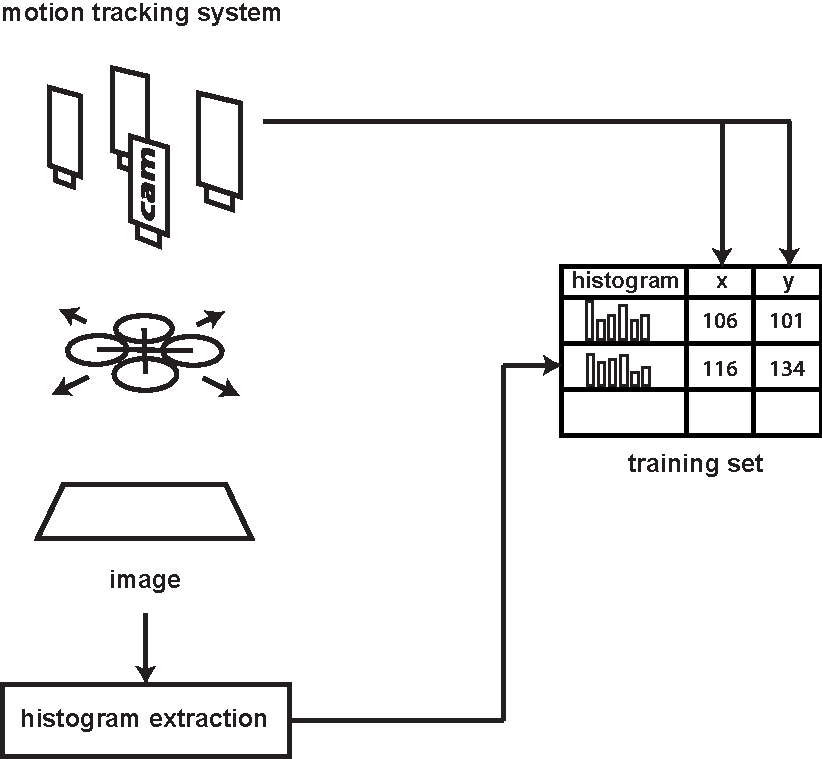
\includegraphics[width=0.56\columnwidth]{overview_new}
\caption{{Training dataset generation if the motion tracking system is
    used. The texton histograms of the camera images during flight are
    extracted and aligned with the highly accurate position estimates
    of the motion tracking system. The result is a high-quality
    training set of texton histograms and corresponding
    $x,y$-positions.%
  }}
\end{center}
\end{figure}

\begin{figure}[h!]
\begin{center}
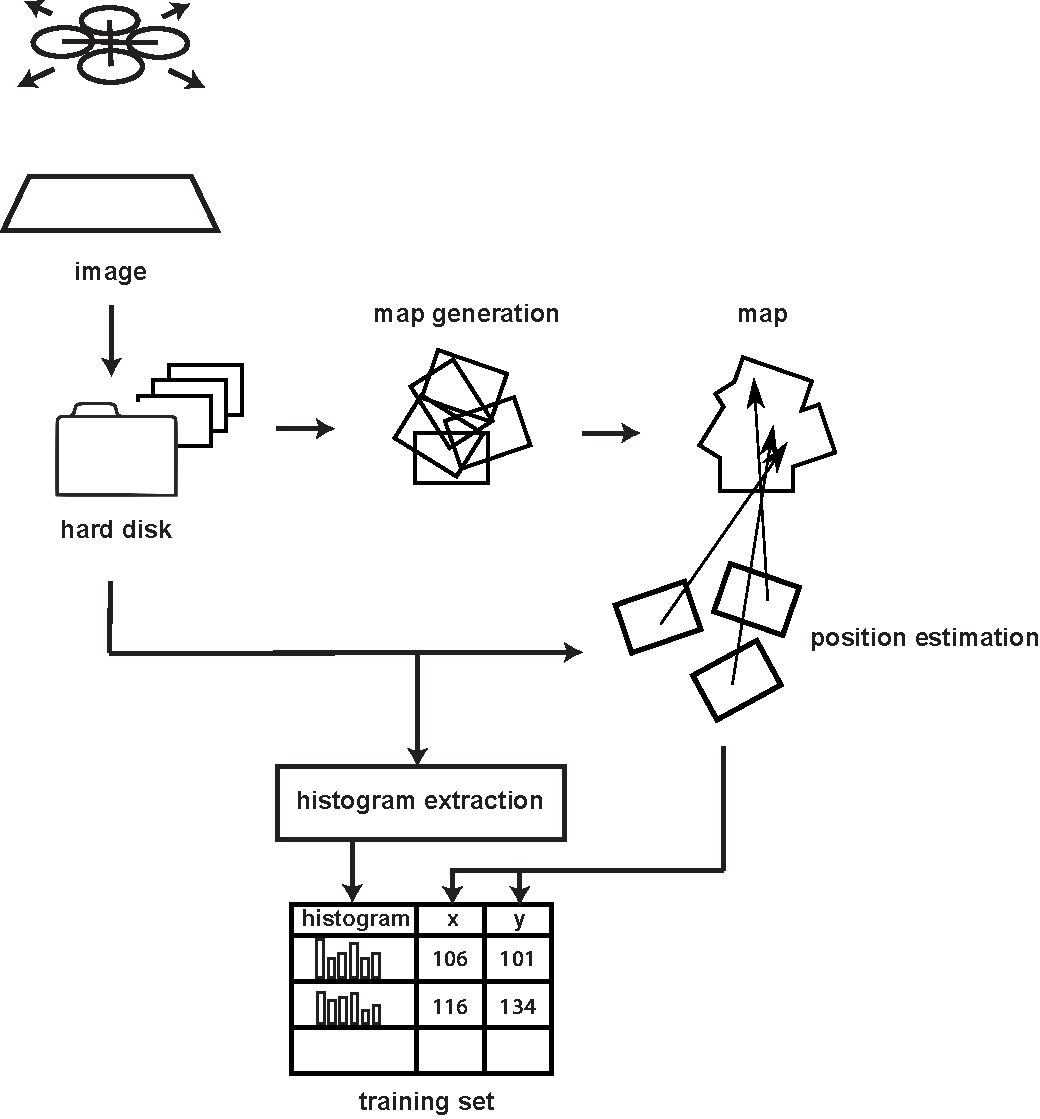
\includegraphics[width=0.7\columnwidth]{overview_sift}
\caption{{\label{fig:overview} The figure illustrates the workflow of
    the proposed approach. After obtaining images from an initial
    flight, the recorded images are stitched together to create an
    orthomap. The same images are used to detect and describe their
    keypoints using \textsc{Sift}, followed by finding a homography
    between the keypoints of the flight images and the orthomap. The
    center of the homography is used as $x, y$ coordinate for labeling
    the training set. Additionally, the number of detected matches is
    saved for the corresponding $x, y$ estimate. Each image of the
    initial flight data set can be used and a fixed amount of small
    $6\times6$ pixel image patches can be extracted. These can be
    labeled with the nearest texton, using a distance measure, for
    example, Euclidean distance. Finally, a classifier can be trained
    using texton histogram as feature vector and the corresponding
    $x, y$ coordinate as target value. This process allows shifting
    computational burden of the keypoint detection and homography
    finding to a faster machine learning approach.%
  }}
\end{center}
\end{figure}

\begin{figure}[h!]
\begin{center}
\includegraphics[width=0.7\columnwidth]{comparison}
\caption{{\label{fig:comparison}
Comparison of an unmodified Parrot AR.Drone.2.0 (left) and a
    modified version (right). The modified one was equipped with an
    Odroid XU-4 single board computer, a Logitech C525 HD camera, a
    WiFi module, and a USB connection between the Odroid board and the
    AR.Drone.2.0 flight controller.%
}}
\end{center}
\end{figure}

\section{Pillar III: Map evaluation}
\label{sec:mapeval}

\subsection{Synthetic Data Generation}
\label{sec:syntheticdatageneration}

In the scope of this thesis, an application to simulate different
camera positions during flight was created. It generates synthetic
image patches based on perspective transformations of a map
image. Examples of generated images are displayed in
Figure~\ref{fig:montage}. The application allows for comparing and
predicting the performance of different maps. The software is written
in C++ and OpenCV~3.0.0.

The software is able to generate a specified amount of image patches
using random values for rotational angles, translational shifts, as
well as blur, contrast and brightness intensity. The values are
sampled from different probability distributions, see
Table~\ref{tab:distributions} for a summary. An additional graphical
user interface (GUI) displays the result of applied transformations
and saves the generated images.

To simulate camera movements in 3D space, a 2D to 3D projection of the
image is performed first. Then, by building separate rotation matrices
$R_x$, $R_y$, and $R_z$ around the axes $x$, $y$, and $z$, the
rotations can be performed separately. Next the rotation matrix $R$ is
created by multiplying the separate matrices, i.e.,
$R = R_x \times R_y \times R_z$. The 3D translation matrix is
multiplied by the transposed rotation matrix. This step is crucial to
rotate the \emph{camera model} and not the image itself. Finally,
after performing all steps, a projection from 3D space to 2D is
applied, to obtain the transformed image.

\begin{table}[h!]
  \centering
  \begin{tabular}{llllll}
    \toprule
    \multicolumn{6}{c}{Distribution}                                                         \\
    \multicolumn{3}{c}{Uniform ($\mathcal{U}$)} & \multicolumn{3}{c}{Normal ($\mathcal{N}$)} \\
    \cmidrule(r){1-3}\cmidrule(r){4-6}
    Parameter                                   & Min   & Max   & Parameter  & M    & STD    \\
    \cmidrule(r){1-3}\cmidrule(r){4-6}
    Yaw                                         & $-5$   & $5$ & Roll       & $90$ & $3$    \\
    Translation X                               & $-800$ & $800$ & Pitch      & $90$ & $4$    \\
    Translation Y                               & $-500$ & $500$ & Brightness & $2$  & $0.1$  \\
    Height                                      & $100$ & $700$ &            &      &        \\
    Blur                                        & $1$   & $10$  &            &      &        \\
    Contrast                                    & $2$   & $3$   &            &      &        \\
    \bottomrule
  \end{tabular}
  \caption[Distributions for the different
  parameters of the synthetic data augmentation tool.]{The table shows the used distributions for the different
    parameters of the synthetic data augmentation tool.}
  \label{tab:distributions}

\end{table}

\begin{figure}[h!]
\begin{center}
\includegraphics[width=0.7\columnwidth]{samples}
\caption{{\label{fig:montage} 
Six images generated by the synthetic data generation tool.%
}}
\end{center}
\end{figure}

\begin{figure}[h!]
\begin{center}
\includegraphics[width=0.672\columnwidth]{camera_model}
\caption{{Camera model for the synthetic flight.%
}}
\end{center}
\end{figure}

\subsection{Evaluation Scheme}
\label{sec:evaluationscheme}

The performance of the proposed method depends on the environment it
is used in: obviously, a texture-rich environment without repeating
patterns will be better suited than an uniformly colored
environment. Ideally, one would like to know if the proposed method is
able to work in a given environment. Therefore, we propose an
evaluation scheme for given maps. This scheme assigns a global fitness
value to a given map, proportional to the expected accuracy it is
expected to achieve in the physical world. The evaluation scheme
allows to inspect the given map and to detect regions that are
responsible for the overall fitness value. The evaluation of a map is
difficult, since the obtained histograms during a real flight depend
on many factors: motion blur, distance to the map and rotations
proportional to the map.

In the first step of the map evaluation procedure, $N$ different
patches of a given map are generated using the tool \emph{draug}
(Section~\ref{sec:syntheticdatageneration}). We propose the following
global loss function ($L$) for evaluating a given map ($\mathcal{M}$):
\begin{align}
  L(\mathcal{M}) &= \sum_{i = 1}^{N} \sum_{j = 1}^{N} \ell(d_a(h_i, h_j), d_e(h_i, h_j))
\end{align}
\begin{align}
  \ell(x, y) &= x - y\\
  d_a(h_i, h_j) &= \text{CS}(h_i, h_j)\\
  d_e(h_i, h_j) &= f_X(pos_i \mid \mu, \Sigma) = f_X(x_i, y_i \mid \mu, \Sigma)\\
\end{align}
\begin{align}
\mu = pos_j = (x_j, y_j)\\
\Sigma =
  \begin{bmatrix}
    \rho & 0\\
    0 & \rho\\
  \end{bmatrix}
\end{align}
The cosine similarity (CS) is:
\begin{align}
CS(h_i, h_j) = \frac{h_i^Th_j}{||h_i||\,||h_j||}
\end{align}
The cosine similarity has the convenient property that its values are
bounded between $-1$ and $1$. In the present case, since the elements
of $h_i$ and $h_j$ are non-negative, it is even bounded between $0$
and $1$. The function $f_x$ describes the non-normalized probability
density function of the normal distribution:
$f_X(x) = e^{- \frac{(x - \mu)^2}{2 \sigma ^ 2}}$. This function is
also bounded between $0$ and $1$, which makes the functions $f_X$ and
$CS$ easily comparable.

The idea behind the global loss function $L$ is that histograms in
closeby areas should be similar and the similarity should decrease the
further away two positions are. This is modeled as a 2-dimensional
Gaussian with zero covariance. The variance is depended on the desired
accuracy ($\rho$): the lower the variance, the more punctuated a
certain location is but also the higher the risk that a totally wrong
measurement occurs. The following visualization are based on color
histograms (and not texton histograms) for easier visual analysis.

In future research, the ``bad regions'' could be optimized using an
optimization approach such as an evolutionary algorithm. It also
allows to show the similarities for a fixed position, and the loss for
a fixed positions based on the expected similarity and the actual
similarity.

\begin{figure}[h!]
\begin{center}
\includegraphics[width=1\columnwidth]{local_loss}
\caption{{TODO: add colorbar! Heatmap colors shows losses per region
    (smoothed using a Gaussian filter). Ideal histogram similarity for
    a given position. Histograms taken at positions close to
    $\textbf{x} = (400, 300)$ should be similar to this histogram. The
    further away the position of a certain histogram, the lower the
    ideal similarity should be.%
  }}
\end{center}
\end{figure}

\chapter{Analysis}
\label{chap:analysis}

In this chapter, the setup of the conducted experiments is
presented. We examine different parameter choices in Experiment~1 to 6
in on-ground experiments using recorded data. Afterward, the found
parameters are used to show the validity during flight in
Experiments~7 and 8. The experiments were conducted in TU Delft's
CyberZoo---an indoor flight arena of size
$w \times l \times h = 10\,m \times10\,m \times 7\,m$, with relatively
constant lighting settings due to primarily artificial lighting.

The choice of the parameters is dependent on the environment and the
size of the training dataset. Therefore, there is no general optimal
parameter. Instead, the parameters have to be adapted to the
particular environment. Since the proposed algorithm is intended for
known environments, this is always possible.

\section{Analysis -- Determining the Number of Textons}
\label{sec:numtextons}

The developed framework allows to tune the computational complexity by
modifying the number of extracted image samples. To increase the speed
of the algorithm, the goal is to use as few samples as possible. To
determine a suitable number of extracted samples, in this experiment,
the average cosine similarity between $D = 20$ datasets of histograms
is compared. Each dataset consists of $N = 10300$ histograms. The
independent variable is the number of extracted image patches $M$. The
histograms were generated using the same images. Due to the random
sampling of the extracted image patches, the histograms of each
datasets will differ. This deviation will be measured using the cosine
similarity. Therefore, each of the $D$ datasets was compared to all
the other $D - 10$ datasets and the average cosine similarity was
determined as well as the standard deviation of the cosine similarity
was measured. Comparing the cosine similarity between the histograms
has the advantage that the number of samples can be determined
independent of a specific task.


Figure~\ref{fig:cosine} displays the cosine similarity of histograms
as a function of the number of samples and the corresponding standard
deviations.

\begin{figure}[h!]
\begin{center}
\includegraphics[width=0.336\columnwidth]{samples_vs_similarity}
\caption{{\label{fig:cosine} Cosine similarity of histograms as a
    function of the number of samples \emph{Right}: Standard deviation
    of cosine similarity in relation to the number of samples. The
    squares indicate the positions at which the dependency was
    evaluated.%%
  }}
\end{center}
\end{figure}


\section{Analysis -- Setting the Baseline for $k$-NN and determining
  $k$}
\label{sec:detk}

In a standard setting, the training error $\epsilon_t$ of a
$k$=1-nearest neighbor algorithm is $\epsilon_t = 0$ because the
nearest neighbor of the sample will be the sample itself, given that
each feature vector is unique. However, in this scenario, we deal with
random sampling such that each image will be represented by a slightly
different histogram each time the histogram is extracted.

\begin{figure}[h!]
\begin{center}
\includegraphics[width=0.7\columnwidth]{map_rotated}
\caption{{\label{fig:mapexp} The created map that was stitched
    together using 445 images. A non-mapped area in the middle of the
    map can be seen, which is a result of the set flight path. An
    image distortion can be seen at the right-hand side, where the
    landing spot sign appears twice, while in reality, only one circle
    was visible.%
  }}
\end{center}
\end{figure}

\begin{figure}[h!]
\begin{center}
\includegraphics[width=0.448\columnwidth]{SIFT_vs_OptiTrack}
\caption{{\label{fig:flightpath} The estimates of the homography
    method compared to the ground truth of the motion tracking system.
    TODO: Legend%
  }}
\end{center}
\end{figure}

\begin{table}[H]
  \centering
  \begin{tabular}{lrrr}
    \toprule
    & x-position & y-position\\
    \midrule
    Error in $cm$ & 31 & 75\\
    STD in $cm$ & 73 & 369\\
    \bottomrule
  \end{tabular}
  \caption[Error statistics homography method.]{Error statistics for the homography method.}
  \label{tab:homoerror}
\end{table}


\section{Experiment -- Motion tracking system for Stabilization,
  Texton-based Approach for estimation}

\subsection{Training Set based on Motion Tracking System}
\label{sec:experiment-real}

In this experiment, a fixed route was set using the ground control
station. While the stabilization and guidance were performed using the
motion tracking system, the position estimates were performed onboard
of the MAV using the texton-based approach. The Euclidean distances
between the estimates of the motion tracking system and the
texton-based approach were measured separately for the $x$- and
$y$-direction. The experiment uses the particle filter and the textons
only. The training dataset was composed of 500 images recorded at an
height of approximately 1\,m, recorded in the time span of one hour
before the experiment. The corresponding $x,y$-coordinates were
obtained from the motion tracking system.

\begin{table}[H]
  \centering
  \begin{tabular}{lrrr}
    \toprule
    & x-position & y-position\\
    \midrule
    Error in $cm$ & 46 & 54\\
    STD in $cm$ & 56 & 71\\
    \bottomrule
  \end{tabular}
  \caption[Estimates of the texton-based approach]{Estimates of the texton-based approach}
  \label{tab:route}
\end{table}

\begin{comment}
  \begin{figure}
    \includegraphics[width=0.7\textwidth]{route}
    \caption[Estimates of the texton-based approach]{Estimates of the
      texton-based approach}
    \label{fig:route}
  \end{figure}
\end{comment}

\subsection{Training Set based on Homography-finding Method}
\label{sec:traininghomo}

In this experiment, the training dataset was created using the
homography-finding method. Apart from that, the settings are the same
as in Experiment~\ref{sec:experiment-real}.

\section{Experiment -- Triggered Landing}
\label{sec:triggered}

In the triggered landing experiment, the UAV was programmed to land as
soon as its position estimates are in the landing zone. The landing
zone was defined as a circle with a radius of $60\,cm$. The
$x,y$-coordinate of the center of the circle was specified in the
flight plan. A safety criterion based on the variance of particles was
introduced, such that the landing is only performed if the criterion
holds. The criterion parameter was set to 60\,cm in both $x-$ and
$y$-direction. The experiment was conducted on a $5m \times 5m$ map
and the ground truth was based on the position data from the motion
tracking system. The training dataset was composed of 500 images
recorded at an height of approximately 1\,m, recorded in the time span
of one hour before the experiment. Table~\ref{tab:targetlanding} shows the results of the triggered
landings. Four out of six landings were correctly performed in the
landing area. The mean distance of outliers was 16\,cm.
\begin{table}[H]
  \centering
  \begin{tabular}{lrrr}
    \toprule
    & x-position & y-position\\
    \midrule
    Error in $cm$ & TODO & TODO\\
    STD in $cm$ & TODO & TODO\\
    \bottomrule
  \end{tabular}
  \caption[Triggered landings]{Results of the triggered landings}
  \label{tab:targetlanding}

\end{table}


\section{Experiment -- Determining the Frequency}

The frequency of the proposed algorithm is determined by varying the
number of samples in the texton-based approach, the number of textons,
and the number of particles of the particle filter.

\section{Experiment -- Comparing different possible maps}

For the map comparison, 50 possible maps have been collected using the
search term `wallpaper' in Google's image search. This search term was
used, since it is (i) a general term, without any specific image
categories, (ii) wallpapers are likely to have a high resolution, and
(iii) wallpapers are likely to be visually pleasant since they are
often used as desktop backgrounds. The criteria for the images were
that their minimum resolution was $1920 \times 1080$. Images with a
higher resolution were converted to $1920 \times 1080$.  For each
image, we generated 1000 random image patches using the simulation
method described in Section~\ref{sec:syntheticdatageneration},
followed by the histogram extraction method. This yielded a labeled
dataset of histograms and corresponding positions. For each map, we
determined the expected overall loss based on the method described in
Section~\ref{sec:syntheticdatageneration}. The compared maps were then
sorted according to their estimated loss.

%Three of the compared maps---the
%best performing, the one with median performance, and the worst
%performing---were printed on A0 paper to test the performance in the
%real world.


In Table~\ref{tab:mapeval}, the results of the map evaluation
procedure for the $N = 46$ maps are shown.

\begin{table}[h]
  \centering
  \begin{tabular}{lr}
    \toprule
    Statistic & Value\\
    \midrule
    mean & 0.57\\
    median & 0.55\\
    standard deviation & 0.14\\
    max & 0.99\\
    min & 0.24\\    
    \bottomrule
  \end{tabular}
  \caption[Map evaluation procedure on synthetic data]{Results of the map evaluation procedure on synthetic data}
  \label{tab:mapeval}

\end{table}

Figure~\ref{fig:minmaximg} shows the map with the highest global loss
value and the map with the lowest global loss value.

\begin{figure}[h!]
\begin{center}
\includegraphics[width=0.7\columnwidth]{lowest_highest}
\caption{{\label{fig:minmaximg}
Image with the lowest loss value; \emph{Right}:
    Image with the highest loss value%
}}
\end{center}
\end{figure}

\chapter{Discussion}
\label{chap:discussion}

In this chapter, the results of the experiments are discussed with
regards to accuracy, frequency, and future improvements. Afterward, in
the General Discussion, the research questions are addressed and
discussed.

The comparison between sub-sampling and full sampling
(Experiment~\ref{sec:numtextons}) has shown that only a small part of
the maximum amount of samples is necessary. In fact,
$\frac{400}{640 \times 480} = 0.13\,\%$ of the maximum amount of
samples suffices to achieve cosine similarities between the texton
histograms larger than $99\,\%$. This set the stage for large
speed-ups during live operation. Additionally, the technique allows
for further speed-ups depending on the processing power of the
platform at hand.

In the real-time position estimation experiment
(Experiment~\ref{sec:experiment-real}), the initial mean error
was rather large: 130\,cm in $x$-direction and 90\,cm in
$y$-direction. A more in-depth analysis revealed that the estimates of
the particle filter were lacking behind the position estimates of the
motion tracking system. This was due to the simple motion model of the
particle filter that was based on Gaussian noise only. By shifting the
estimates of the particle filter by six frames, that is approx. 0.46
seconds at a frequency of 13\,Hz, the error could be reduced to 46\,cm
in $x$-direction and 54\,cm in $y$-direction. This lag can be
addressed by to strategies: (i) slower speed during flight, (ii) a
better or more flexible motion model.

The triggered landing (Experiment~\ref{sec:triggered}) showed a high
accuracy. While most landings were triggered inside the landing zone,
two out of the six landings were outliers. However, their distance to
the landing area were rather small, with an average distance of
16\,cm. A comparison without the safety criterion, showed, that the
criterion can have advantages.

The evaluation of different maps using the synthetic data showed high
differences between the evaluated images. The range of losses from
0.24 to 0.99 underlines the varying suitability of different maps for
the proposed algorithm.
% To visually evaluate the map evaluation technique, a simple map was
% constructed with two repeating tiles.
The
image with the minimum and the one with the maximum loss value based
on their color histogram are shown in Figure~\ref{fig:minmaximg}. The
different patterns of the images are clearly visible: while the image
with the minimum value fulfills the desired properties---closeby areas
have similar color values, distant areas are dissimilar, the image
with the maximum loss is mainly black resulting in similar histograms
all over the place and leading to high loss values. This initial
evidence can be taken to test the predictive power of the evaluation
algorithm for texton histograms.

\section{General Discussion}
\label{sec:generaldiscussion}

In this chapter, the results will be discussed regarding error
statistics, execution frequency, robustness, and scalability. To begin
with, we recapitulate the research questions:

\begin{itemize}
\item R1: Can accurate 2D positions be estimated in real-time, using a
  machine learning-based approach on a limited processor in a
  modifiable indoor environment?
\item R2: Is accurate real-world localization regression or classification
  possible when the training data comprises synthetic data only?
\item R3: Can we predict the goodness of a given map for the proposed
  localization approach?
\end{itemize}

Regarding R1, the conducted experiments provide supportive evidence
that a texton-based machine learning approach is able to accomplish
real-time indoor localization. The proposed algorithm runs with as
frequency of 30\,Hz on a single board computer with limited
CPU. Shifting processing power to an offline training step and relying
on random sampling are the cornerstones for running the algorithm on
processors with limited CPU. Despite the small ratio between extracted
image patches ($s$) and the maximum amount of different image matches
($s*$), the accuracy is hardly affected, and only slightly improves
when incorporating more textons.

Regarding research question R2, the initial idea---to use the
synthetically generated images directly as training data---was not
successful and not further followed up. This might be also the reason
that only few projects have used synthetic images for real-world
phenomena. The reality gap between the synthetic data and real-world
data was huger than expected. Figure~\ref{fig:realitygap} shows an
example of two image patches, one synthetically generated, one taken
with the camera of the MAV. While the patches can be easily identified
as similar for human eyes, the texton maps, where different colors
represent different textons, are dissimilar. Blur, lighting settings,
and camera intrinsics modify low-level features of the image to a too
strong extent. A possible improvement might be to find a mapping from
histograms of synthetic images to histograms of real images, by
mapping 'synthetic textons' to 'real-world textons'.

Referring to R3, we found some initial evidence that the proposed map
evaluation generalizes to the real-world. In contrast to R2, the
generalization from the synthetic data to real-world data is of a
different nature in this case. The requirement here is that maps that
follow the ideal similarity distribution in the synthetically
generated images also follow this distribution after being recorded
with a camera. Or stated differently, for maps with a low loss value,
distant image positions should not have similar histograms using the
synthetic images nor the real-world images.

Despite the overall promising results, we noticed drawbacks of the
proposed approach during the flight tests and directions for future
research.

The accuracy---that is the difference between the estimates of the
motion tracking system and the texton-based approach--- could be
further improved by incorporating more features, for example histogram
of oriented gradients. Additional improvements could be obtained by
investigating further regression techniques, like Gaussian processes
or Bayesian networks that can inherently handle space and time.

The developed method sets the stage for numerous future research
directions and improvements. The current implementation assumes rather
constant height (up to few centimeters) and no angular rotations of
the MAV. While a quadroter can move in every direction without
performing yaw movements, using the MAV on another vehicle could
require arbitrary yaw movements. To limit the complexity of the
dataset, a ``derotation'' of the incoming image could be performed to
align it with the underlying images of the dataset. While the current
approach normalizes each $5\times5$ image patch to unit mean and zero
variance---giving robustness to different lighting conditions---this
procedure could be further extended, for example by using specific
color models.

While the current map evaluation approach used existing fixed images,
it could also serve as a fitness function for an optimization
approach---for example, an evolutionary algorithm---which modifies a
given image. This could allow to find a near optimal solution for a
given regression technique and give insightful view in the underlying
structure of certain regression techniques. While the solution to a
loss value of zero or near zero might be unique and independent of the
original image, a higher loss value might change the initial image
only to a certain extent, yielding an ``improved version of the
image'', which is better suited for the proposed algorithm.

The presented software \emph{draug} generates image patches based on
drawing samples from parametric distributions only. This was motivated
by the fact that an ideal map should be independent of previous
estimates and based on single images only---ideally requiring no
filtering. In the future, the possibility to set flight routes by
setting way points above an image could be included. This would allow
to test the ability of the particle filter on synthetic flights.

\begin{figure}[h!]
\begin{center}
\includegraphics[width=0.448\columnwidth]{realitygap}
\caption{{\label{fig:realitygap}
Exemplifying the reality gap. \emph{Top left}: image patch generated using draug. \emph{Top
      right}: image patch taken with the MAV's camera after printing
    the patch. \emph{Below left}: texton image of the synthetic
    image. \emph{Below right}: Texton image of the real image. The
    texton images shows that corresponding regions get classified into
    different textons, resulting in different histograms. This makes
    the transfer from the synthetic data to the real world difficult.%
}}
\end{center}
\end{figure}

The shift of the processing power could be further amplified by using
a different regression technique. In the current implementation using
$k$-NN regression, larger training data sets are penalized due to a
greater prediction time. However, the choice of a different regression
technique is not as straightforward as it might seem. The technique
should be able to output multiple predictions, since certain map
regions might be ambiguous.

The presented approach is a vision-only approach. This makes it robust
to external disruptions such as magnetic fields and reduces the amount
of points of failure. Additionally, the approach can be used on
different devices, such as handheld cameras. Still, future
developments could incorporate data from the inertial measurement unit
(IMU) in the particle filter's motion model.

Additionally, the time complexity of the algorithm can be further
reduced with the aim of running the algorithm on fly-sized
MAVs. Depending on the target platform, parallelization or threading
could be used on multi-core systems to simultaneously compute texton
histograms, make predictions and run the particle filter.

% Currently, the computationally most complex part is the XXX.


\chapter{Conclusion}
\label{chap:conclusion}

This thesis presented a novel approach for lightweight indoor
localization of MAVs. We pursued an onboard design without the need of
an additional ground station to foster flexibility and autonomy. The
conducted on-ground and in-flight experiments underline the real-world
applicability of the system. Promising results were obtained for
waypoint navigation, accurate landing, and stable hovering in the
indoor environment. The
used approach is based on three pillars.\\
The first pillar shifts computational effort from the flight phase to
an offline preprocessing step. This provides the advantages of
sophisticated algorithms, without affecting performance during flight.
The second pillar states that during flight the MAV lightweight
algorithms should run with low-performing processors. These algorithms
should be able to trade off speed with accuracy. This allows to use
them on a wide range of models, from pico-drones to MAVs with a
wing-span of over one meter. Examples of these adaptable algorithms
are the particle filter and the texton-based approach.  The third
pillar is the known---and possibly---modifiable environment. This
knowledge and flexibility allows to predict the quality of the used
approach. In contrast to SLAM frameworks, in which the task is to
simultaneous mapping and localization, the proposed approach is
intended for various repetitive indoor activities.


The developed algorithms set the stage for absolute localization in
various GPS-denied environments, such as homes, offices, or factory
buildings. While the used platform for this project was the Parrot
Bebop Drone, the characteristics of the proposed system generalize to
smaller MAVs in a flexible and innovative way.  We hope that our
indoor localization approach will pave the way for various
applications, such as delivery, search and rescue, or surveillance to
support human operators in everyday life.

\printbibliography

\end{document}

